\begin{frame}{Rendering und Phsyik}
\end{frame}
\begin{frame}{Darstellung des Spielfeldes}
\begin{itemize}
	\item Hintergrundfarbe Dunkel-Grün mit der OpenGL ClearColor
	\item Löcher und Kugeln mit Triangle-Fan
\end{itemize}
\end{frame}
\begin{frame}{Triangle-Fan}
\begin{itemize}
	\item Struktur aus Dreiecken
	\item Mittelpunkt $c$
	\item Radius $r$
	\item Auflösung $k$ ist die Anzahl der Dreiecke, aus denen unser Kreis hinterher besteht
\end{itemize}
\end{frame}
\begin{frame}{Triangle-Fan}
Berechnung:
\begin{itemize}
	\item [1.] Berechnen vom Winkel $\delta = \frac{2 \cdot \pi}{k}$, der den Abstand zwischen den Punkten auf dem Kreis darstellt
	\item [2.] Mittelpunkt $= (0,0)$, Objekt wird später an die Stelle $c$ transformiert
	\item [3.] Erste Punkt auf dem Kreis ist $(r,0)$
	\item [4.] Dreieck wird vollendet mit dem Punkt $	x = \cos (\delta \cdot i) \cdot r$\\
				$y = \sin (\delta \cdot i) \cdot r$, mit $i =$ Anzahl der Iterationen von $i = 0$ bis $k$
	\item [5.] Jeder neu hinzugefügte Punkt wird mit dem Mittelpunkt und dem letzten Punkt auf dem Umriss zu einem Dreieck verbunden
\end{itemize}
\end{frame}
\begin{frame}
\begin{figure}
	\caption{Erstes Dreieck eines Triangle-Fans, i = 1, k = 36}
	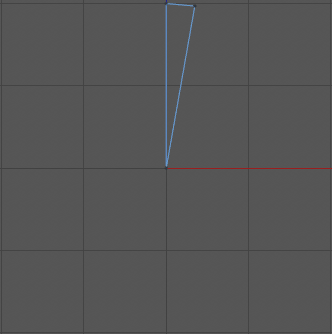
\includegraphics[width =150pt]{bilder/1.png}
\end{figure}
\end{frame}
\begin{frame}
\begin{figure}
	\caption{i = 2, k = 36}
	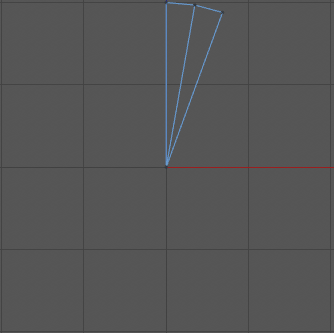
\includegraphics[width =150pt]{bilder/2.png}
\end{figure}
\end{frame}
\begin{frame}
\begin{figure}
	\caption{i = 3, k = 36}
	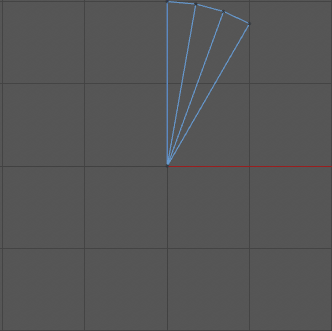
\includegraphics[width =150pt]{bilder/3.png}
\end{figure}
\end{frame}
\begin{frame}
\begin{figure}
	\caption{Vollständiger Triangle-Fan, i = k = 36}
	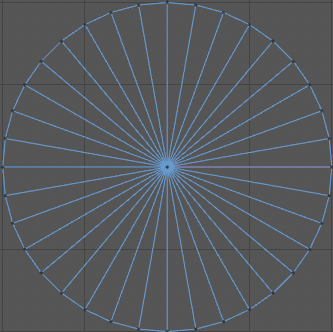
\includegraphics[width =150pt]{bilder/full.png}
\end{figure}
\end{frame}
\begin{frame}{Zwischenstand}
Wir haben nun ein Spielfeld mit Löchern und Kugeln. Jedoch sind die Kugeln noch nicht voneinander zu unterscheiden.
\begin{figure}
	\caption{Spielfeld ohne Texturen}
	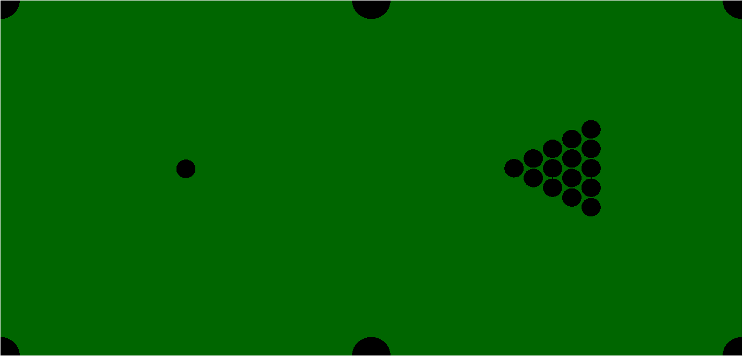
\includegraphics[width=250pt]{bilder/untextured_pool_low.png}
\end{figure}
\end{frame}
\begin{frame}{Texturierung}
Grundkonzepte:
\begin{itemize}
	\item Eine Textur besteht aus Koordinaten auf der u (waagerecht) und der v (vertikal) Achse
	\item Die beiden Achsen sind immer im Bereich $[0,1]$, egal wie groß die Textur ist
	\item Man gibt beim Erstellen von Objekten für jeden Knoten die Texturkoordinaten in u und v an, um sie auf das Objekt abzubilden
\end{itemize}
\end{frame}
\begin{frame}{Texturierung}
\begin{figure}
	\caption{Textur mit u- und v-Achse}
	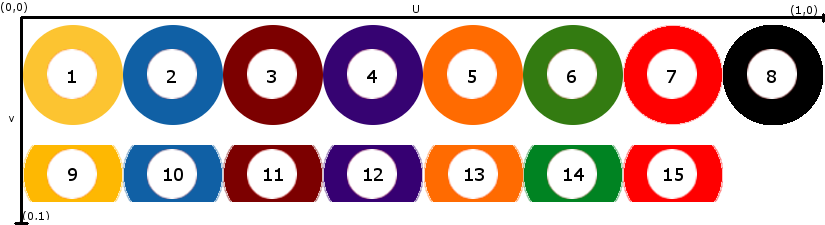
\includegraphics[width=250pt]{bilder/ballsachsen.png}
\end{figure}
Es fällt auf, dass eine Kugel $\frac{1}{8}$ Durchmesser hat auf u, aber $\frac{1}{2}$ auf v
\end{frame}
\begin{frame}{Texturierung}
Wir müssen nun berechnen, welcher Ausschnitt für welche Kugel ist.
	\begin{itemize}
		\item Die Farben sind geordnet auf der Textur und bekommen Werte von 0 bis 7
		\item Die Vollen Kugeln sind in der ersten Reihe und die Halben in der Zweiten und bekommen damit die Werte 0 (voll) und 1 (halb)
		\item Wir können jetzt eine Funktion erstellen, die uns anhand von Farbe und Fülle den Textur Mittelpunkt ausgibt 
	\end{itemize}
\end{frame}
\begin{frame}{Texturierung}
Beispiel: Mittelpunkt der gelben, halben Kugel auf der Textur: \\
	$u = \frac{1}{16} + \frac{1}{8} \cdot 0 = \frac{1}{16}$\\
	$v = \frac{1}{4} + \frac{1}{2} \cdot 1= \frac{3}{4}$ \\
Dabei ist $\frac{1}{16}$ der Radius einer Kugel auf u, und $\frac{1}{4}$ der Radius auf v.
Die Funktion ist dann: \\
$	u(b) = \frac{1}{16} + \frac{1}{8} \cdot c(b), c(b) = \text{Farbe der Kugel}$\\
$v(b) = \frac{1}{4} + \frac{1}{2} \cdot f(b), f(b) = \text{Fülle der Kugel}$\\
\end{frame}
\begin{frame}{Zwischenstand}
Wir haben nun ein fertiges Spielfeld mit Texturierten Kugeln.
\begin{figure}
	\caption{Fertiges Spielfeld}
	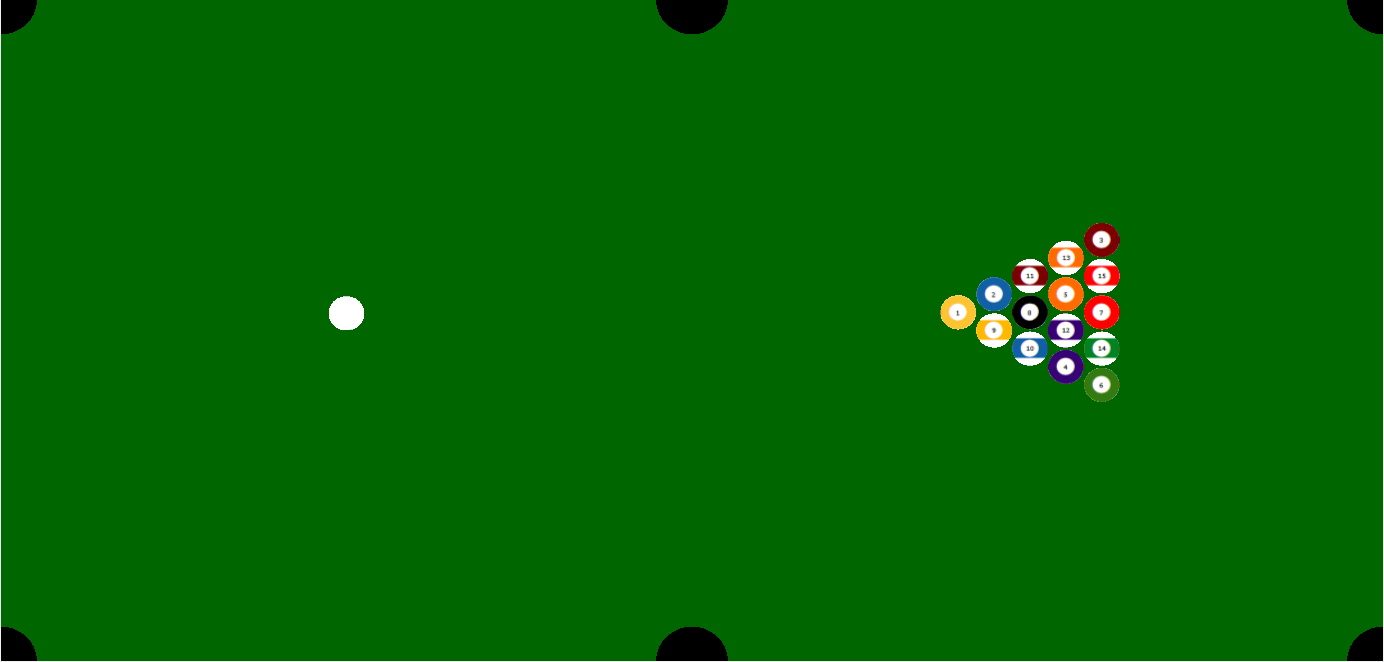
\includegraphics[width=300pt]{bilder/Spielfeld.png}
\end{figure}
\end{frame}
\begin{frame}{Physik}
Die Physik-Berechnungen des Spiels lassen sich aufteilen in 3 Bereiche:
\begin{itemize}
	\item Kollision von Kugel und Wand
	\item Kollision von Kugeln mit anderen Kugeln
	\item Kollision vom Queue mit der weißen Kugel
\end{itemize}
\end{frame}
\begin{frame}{Kollisionen: Kugel mit Wand}
Prinzip sehr einfach:
\begin{itemize}
	\item [1.] Definiere die Wände als Achsenabschnitte: Linke Wand ist $x=0$, rechte Wand $x=w$, obere Wand $y=0$ und untere Wand $y=h$, mit $w = $ Breite des Spielfeldes und $h = $ Höhe des Spielfeldes
	\item [2.] Überprüfen ob eine der Koordinaten der Kugel zusammen mit dem Radius eine der Wände schneidet \\
				z.B. für $r=5$ wäre $x = 5 - r = 0 $ und würde somit die Linke Wand schneiden
	\item [3.] Geschwindigkeit auf der Achse die Geschnitten wurde invertieren, also bei $x=0$ oder $x=w$ wird $vx = -vx$ gesetzt, analog für y
\end{itemize}
\end{frame}
\begin{frame}{Kollisionen: Kugel mit Wand}
Nun fehlen noch die Löcher: 
\begin{itemize}
	\item Wir setzen zusätzliche Bedingungen für die Kollision mit Wänden ein
	\item Wir überprüfen beim Schnitt mit einer der Wände, ob der Ausschnitt auf bei einem Loch liegt 	
\end{itemize}

$vx = \begin{cases}
-vx, & \text{ falls } y \leq (h- l) \land y \geq l, l = \text{Radius eines Lochs}\\
vx, & sonst 
\end{cases}$
Analog für $vy$, nur mit 2 Wandabschnitten auf der X-Achse aufgrund der 3 Löcher auf X. \\
Wenn der Mittelpunkt einer Kugel von der Distanz her weniger weit entfernt ist von dem Mittelpunkt eines Lochs, als der Radius von diesem, dann lassen wir die Kugel verschwinden und zählen sie als Punkt.

\end{frame}

\begin{frame}{Kollision mit anderen Kugeln}
\begin{itemize}
	\item Die Kollision von 2 Kreisen war uns bereits gegeben durch das Airhockey-Spiel.
	\item In Airhockey kollidiert ein Puck mit einem der beiden Schläger und bekommt dadurch eine neue Geschwindigkeit
	\item Der Schläger wird von der Kollision nicht verändert
	\item Wir brauchen aber, dass sich beide Kugeln bei Kollision verändern
\end{itemize}
\end{frame}
\begin{frame}{Kollision mit anderen Kugeln}
Lösung:
\begin{itemize}
	\item Wir berechnen für jede Kugel die Kollision mit jeder anderen Kugel
	\item Das heißt wir nehmen die Methode aus dem Airhockey und nehmen unsere Kugel die sich bewegen soll als Puck und berechnen die Kollision mit allen anderen Kugeln als Schläger
	\item Wenn wir das in beide Richtungen ausführen, sodass jede Kugel sozusagen einmal Schläger und einmal Puck ist, wird jede Kugel von einer Kollision getroffen 
\end{itemize}
\end{frame}
\begin{frame}{Kollision mit Queue}
Die eigentliche Kollision bleibt gleich wie beim Airhockey. \\
\textbf{Problem: Framerate der Kamera} \\
Dadurch, dass unsere Kamera nur ungefähr 25 Bilder pro Sekunde aufnehmen kann, haben wir bei einer schnellen Bewegung des Queue's ein verwischtes Bild, sodass uns die Kollision abhanden kommen kann. \\
Wir müssen also interpolieren, um zu gucken, ob auf dem Weg eine Kollision stattgefunden hat.
\end{frame}